\section{Theorie}
\label{sec:Theorie}
In diesem Versuch wird die Suszeptibilität verschiedener Seltenen-Erd-Verbindungen bestimmt. 
Anschließend werden die gemessenen Werte mit den theoretisch bestimmten Werten verglichen.
Außerdem wird die Filterkurve des dabei verwendeten Selektiv-Verstärkers untersucht. 
\\
\subsection{Die magnetische Suszeptibilität}
Die magnetische Suszeptibilität $\chi$ gibt an, wie gut ein Material in einem externen Magnetfeld magnetisierbar ist.
Die Magnetisierung $\vec{M}$ des Materials lässt sich in Abhängigkeit von der magnetischen Feldstärke $\vec{H}$, der Suszeptibilität $\chi$ und der 
Induktionskonstanten $\mu_0$ als
\begin{equation}
    \vec{M}=\mu_0 \chi \vec{H}
\end{equation}
darstellen. Dabei ist die Suszeptibilität nicht konstant, da sie sowohl von $\vec{H}$ als auch von der Temperatur $T$ abhängt. Unter Raumtemperatur und bei kleinen Magnetfeldern $\lvert \vec{B} \rvert <\SI{1}{\tesla}$
kann die Suszeptibilität näherungsweise als konstant angesehen werden. Mit Hilfe der Suszeptibilität lassen sich zwei Gruppen von Materialien unterscheiden.
Stoffe mit $\chi<0$ sind diamagnetisch und werden in einem äußeren Magnetfeld entgegengesetzt zu der Feldrichtung magnetisiert. Hat ein Stoff eine Suszeptibilität $\chi>0$ ist der Stoff
paramagnetisch. Die Magnetisierung verläuft mit der Feldrichtung des äußeren Felds, sodass das innere Magnetfeld des Stoffvolumens stärker ist. Die Suszeptibilität
ist antiproportional zur Temperatur, sodass die Magnetisierung bei zu hohen Temperaturen verschwindet.
\\
\subsection{Berechnung der Suszeptibilität}
Zunächst muss der Zusammenhang zwischen dem atomaren Drehimpuls und dem daraus resultierenden magnetischen Moment hergestellt werden und dann über alle möglichen Orientierungen relativ zu einem äußeren
Feld aufsummiert werden. Dabei setzt sich der Gesamtdrehimpuls $\vec{J}$ aus dem Bahndrehimpuls der Elektronenhülle $\vec{L}$, dem Gesamtspin $\vec{S}$ und dem für den Paramagnetismus vernachlässigbaren Kerndrehimpuls zusammen.
Dem Bahndrehimpuls und dem Gesamtspin können durch Erkenntnisse aus der Quantenmechanik die magnetischen Momente
\begin{align}
    \vec{\mu_\text{L}} &= - \frac{\mu_\text{B}}{\hbar} \vec{L} \ , \\
    \vec{\mu_\text{S}} &= - g_\text{S}\frac{\mu_\text{B}}{\hbar} \vec{S}
\end{align} 
zugeordnet werden. Bei $\mu_\text{B}$ handelt es sich um das Bohrsche Magneton und bei $g_\text{S}$ um das gyromagnetische Verhältnis des freien Elektrons.
Mit den Quantenzahlen der Drehimpulse $\vec{J}$ und $\vec{L}$ und des Spins $\vec{S}$ ergibt sich für die Beträge
\begin{align}
    \lvert \vec{\mu_\text{L}} \rvert &= - \mu_\text{B} \sqrt{L\left(L+1\right)} \, , \\
    \lvert \vec{\mu_\text{S}} \rvert &= - g_\text{S} \mu_\text{B} \sqrt{S\left(S+1\right)} \, .
\end{align}
\begin{figure}
    \centering
    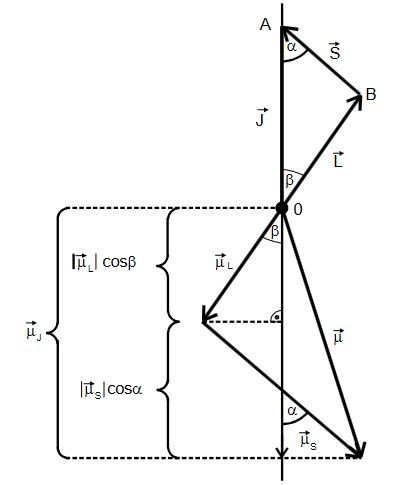
\includegraphics[scale=0.4]{pics/Vektor.png}
    \caption{Vektordiagramm aus den Drehimpulsvektoren einer Elektronenhülle und den daraus resultierenden magnetischen Momenten. \cite{v606}}
    \label{fig:VE}
  \end{figure}
Aus Abbildung \ref{fig:VE} lässt sich die Beziehung
\begin{equation}
    \lvert \vec{\mu_\text{J}} \rvert = \lvert \vec{\mu_\text{S}} \rvert \cos(\alpha) + \lvert \vec{\mu_\text{L}} \rvert \cos(\beta)
\end{equation}
herleiten. Mit Hilfe des Cosinussatzes kann näherungsweise der Lande-Faktor
\begin{equation}
    \lvert \vec{\mu_\text{J}} \rvert \approx \mu_\text{B} g_\text{J} \sqrt{J\left(J+1\right)}
\end{equation}
abgeleitet werden. Dabei ist der Ausdruck $g_\text{J}$ als
\begin{equation}
    g_\text{J} \coloneq \frac{3 J \left(J+1\right) + \{S\left(S+1\right)-L \left(L+1\right)\}}{2J\left(J+1\right)}
\end{equation}
definiert.
Zu beachten ist die Richtungsquantelung aus der Quantenmechanik, welche besagt, dass der Winkel zwischen äußerem Magnetfeld und $\vec{\mu_\text{S}}$
nicht beliebig ist, sondern die Beziehung
\begin{equation}
    \mu_{\text{J}_Z}=- \mu_\text{B} g_\text{J} m
\end{equation}
für die Z-Komponente des magnetischen Moments $\vec{\mu_\text{J}}$ gilt. Die ganzzahlige Größe m wird Orientierungsquantenzahl genannt und kann die Werte $-\text{J}$ bis J annehmen.
Dadurch sind 2J+1 Einstellungen für den Winkel möglich. 
Über alle Einstellungen und deren Wahrscheinlichkeiten summiert, ergibt sich
\begin{equation}
    \chi=\frac{\mu_0 \mu_\text{B}^2 g_\text{J}^2 N J \left(J+1\right)}{3 k T} \label{eqn:sustheo}
\end{equation}
für die Suszeptibilität. Dabei ist $N$ die Momentanzahl pro Volumeneinheit, $k$ die Boltzmannkonstante und $T$ die Temperatur.
\\
Es ist bekannt, dass Verbindungen, die Ionen Seltener Erden enthalten, einen starken Paramagnetismus aufweisen.
Diese Ionen besitzen große Drehimpulse, aufgrund der in der 4f-Schale lokalisierten Elektronen. 
Die Anordnung  der  Elektronen  in  der  unabgeschlossenen  4f-Schale  und  der  daraus  resultierende  Gesamtdrehimpuls  $\vec{J}$  werden  durch  die  sogenannten  Hundschen  Regeln  festgelegt.
Diese lauten.
\begin{itemize}
    \item Die Spins $\vec{s_\text{i}}$ kombinieren zum maximalen Gesamtspin $\vec{S}= \sum \vec{s_\text{i}}$ der nach dem Pauli-Prinzip möglich ist.
    \item Die Bahndrehimpulse $\vec{l_\text{i}}$ summieren sich nach dem Pauli-Prinzip zum Maximaldrehimpuls $\vec{L}=\sum \vec{l_\text{i}}$.
    \item Der Gesamtdrehimpuls ist $\vec{J}=\vec{L}-\vec{S}$, wenn die Schale weniger als halb und $\vec{J}=\vec{L}+\vec{S}$, wenn die Schale mehr als halb gefüllt ist.
\end{itemize}
\subsection{Bestimmung paramagnetischer Suszeptibilitäten}
Zur Bestimmung einer Suszeptibilität kann eine Brückenschaltung, wie in Abbildung \ref{fig:sus} zu sehen ist, verwendet werden. 
Dabei basiert die Messung auf einer Induktivitätsdifferenz $\symup{\Delta}L$ zwischen einer mit einem Paramagneten befüllten und einer unbefüllten Spule.
Diese Spulen sollten unbefüllt eine möglichst ähnliche Induktivität besitzen.
Für hohe Spannungsfrequenzen $\omega^2 L^2 >> R^2$ gilt die Beziehung
\begin{equation}
    \chi\left(\omega \to \infty \right) =\frac{4 F U_\text{Br}}{Q U_\text{Sp}}
    \label{eqn:chil}
\end{equation}
mit dem Spulenquerschnitt $F$, den Probenquerschnitt $Q$, der Speisespannung $U_\text{Sp}$ und der Brückenspannung $U_\text{Br}$.
\begin{figure}
    \centering
    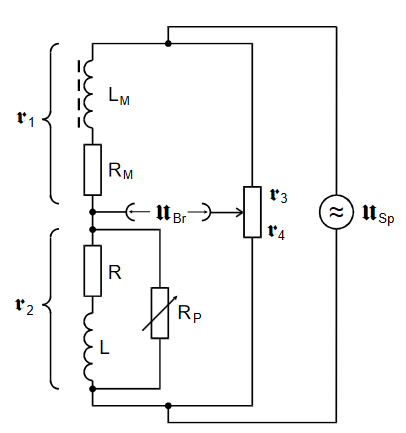
\includegraphics[scale=0.4]{pics/sus.png}
    \caption{Brückenschaltung für eine Suszeptibilitätsmessung. \cite{v606}}
    \label{fig:sus}
  \end{figure}
An der Brückenschaltung kann ebenso mit Hilfe der Abgleichbedingung die Beziehung
\begin{equation}
    \chi = \frac{2 \symup{\Delta}R F}{R_3 Q}
    \label{eqn:chir}
\end{equation}
für die Suszeptibilität genutzt werden. Dabei ist $\symup{\Delta}R$ die Differenz der Potentiometereinstellungen.